\chapter{General Description}
\label{chap:gendesc}
In this chapter we discuss the relation of this project to the ``outside world'': if there are any related projects running currently and if there were related projects in the past. Then, the purpose of the \applicationname{} and the environment in which it operates are discussed. After that, its relation to other systems is covered. Finally, some general constraints are described and a description of the logical model is given.

\section{Relation to current projects}
\label{sec:curproj}
%The context of this project in relation to other current projects
No other current projects are related to \projectname{}.

\section{Relation to predecessor and successor projects}
\label{sec:predsuc}
%The context of this project in relation to past and future projects
\projectname{} has multiple predecessor projects. These projects resulted in multiple Matlab\footnote{\url{http://www.mathworks.nl/products/matlab/}} tools that are available on the client's web page \cite{clientpage}. \projectname{} will combine some of the functionality of these tools into a mobile web application. \projectname{} will be developed in such a way that the client can easily extend the application with new mixers. When the development of \projectname{} is complete, \projectname{} is no longer responsible for the application after the final deliverable produced in the SEP project. This means that the client may change, add or remove the application's functionality.

\section{Function and purpose}
\label{sec:functpurp}
%A general overview of the function and purpose of the product
\projectname{} is an application that serves as an educational tool for anyone who wants to gain a deeper understanding of the process of mixing in general, and in particular for students at the TU/e. By interacting with the application, users can quickly and easily find out what the effects of a certain mixer and mixing protocol on an initial distribution are. The user can thus obtain a better understanding about the way this mixer functions. \projectname{} may also be used as a quick and convenient way to observe whether a mixing protocol renders good or bad mixing results. 

\section{Environment}
\label{sec:env}
%Hardware and operating system of target system and development system
\projectname{} is a web application that is developed primarily for use on mobile devices. This means the application will mostly be accessed through web browsers on smartphones and tablets. It is expected that the application will mostly be used on iPhones and iPads. Therefore, \projectname{} must support iOS Safari version 6.0 and above. Furthermore, \projectname{} should support Firefox version 20 and above, and Google Chrome version 26 and above. Lastly, if time permits, \projectname{} could also support Internet Explorer version 10 and above, Opera version 12.1 and above, and Safari version 6.0 and above.

To support the significant share of smartphones and tablets that run on Android, \projectname{} should run on devices running on Android version 4.0 and higher. Lastly, if time permits, \projectname{} could also run on devices running on Windows 8.

The hardware used by the users must be able to run at least one of the supported operating systems and browsers. Also, the application obviously works better on screens that have a diagonal of at least about 4 inches and a resolution of at least about 540x960 pixels - the larger the screen, the easier it is to draw on it (up to a certain maximum, about the size of a desktop monitor with a diagonal of 20 inches). This is because the user draws with their finger and since fingers have a certain size, the screen should be large enough to comfortably draw and see what has been drawn at the same time. On the other hand, when the screen is too big, it costs too much effort to fill up large parts of the mixer.

The application must support the following screen resolutions:
\begin{itemize}
	\item ``Phone portrait'': 540x960 pixels;
	\item ``Phone landscape'': 960x540 pixels;
	\item ``Tablet portrait'': 800x1280 pixels;
	\item ``Tablet landscape'': 1280x800 pixels;
	\item ``Desktop'': 1600x900 pixels.
\end{itemize}

\section{Relation to other systems}
\label{sec:othersys}
The \applicationname{} is an independent system. However, just like every other web application, it is dependent in some way on the browser. That is, the correct (according to the HTML standard\footnote{\url{http://www.whatwg.org/}}) rendering of the web page is done by the browser. Of course, the application will be tested in multiple browsers and built in such a way that it displays correctly in as many browsers as possible.

\section{General constraints}
\label{sec:genconst}
The user interface should be suitable for mobile devices, so it will be easy to share the visualised results with other people, and to quickly try out new ideas for mixers wherever the user may be.

We assume that the server can compute the displacement of fluids reasonably fast\footnote{Refer to chapter 6 of the ADD \cite{add} for exact requirements.}, so the mixing run can be executed quickly. When the new concentration distribution has been computed, this concentration distribution is sent back to the client device along with a metric to indicate the performance of the mixer. The results are then visualised on the client's device.

As we do not want to be locked to one specific type of device, we have chosen to design a cross-platform solution. While this means that desktop PCs should also be able to run the application, we do not actively support such devices. We will instead concentrate on mobile devices.

It should be possible to save mixing runs on the client device for later reference. For each saved run, we store the initial distribution, the mixer and protocol
used, the resulting fluid distribution and the resulting performance metric.

\section{Model description}
\label{sec:moddesc}
On a very high level, the architecture of the \applicationname{} can be divided into different tiers communicating through communication channels. A graphical representation of the relation between tiers and channels can be found in figure \ref{fig:tierchannel}.

\subsection{Client tier}
\label{sec:clienttier}
Of the Client tier, there are an arbitrary number of instances. These instances are the physical machines of the users of the \applicationname{} (phones, tablets, laptops, desktops).

\subsubsection{Client Browser and Client Persistence}
\label{sec:clientbrowser} 
Each Client instance runs a Client Browser (one of the browsers as specified in section \ref{sec:env}) and has a persistent storage facility (Client Persistence). The Client Browser can use this facility to store data that is specific to the user and does not need to be stored in a central location. The Client Browser provides the user with a Graphical User Interface. All interactions of the user with the application are performed through this GUI.

\subsection{Application Server tier}
\label{sec:aplicationserver}
The Application Server is a physical machine maintained by the system administrator of the application. It is used to distribute the application and provide services to the application.

\subsubsection{HTTP Server}
\label{sec:httpserver}
The application is distributed on demand to the Client instances using HTTP by the HTTP server. The HTTP server is a piece of software that responds to requests by serving a file from a static collection of content, which is used to serve the actual application.

\subsubsection{Application Service}
\label{sec:applicationservice}
Whenever centralised data or a simulation is required by the application running on a Client, this is handled by the Application Service in response to a request from the Client Browser. This service is responsible for communicating any simulations and their results and also for serving data from the persistent storage. Data from the persistent storage can be a list of mixers for example.

\subsection{Application Persistence tier}
\label{sec:applicationpersistence}
The Application Service may use a global persistent storage facility in order to store data that needs to be available to all Clients. This storage facility is provided in the Application Persistence tier and is communicated to through the Application Persistence Communication channel. This tier may be on a different physical machine than the Application Server, but in practice, it will likely run on the same hardware.

\subsection{Simulator Server}
\label{sec:simulatorserver}
The simulations that need to be done for the application run on a dedicated machine although in practice, this will likely be the same physical machine as the Application Server.

\subsubsection{Simulator Service and Fortran Module}
\label{sec:simulatorservice}
Whenever a Client wishes to run a simulation, it interfaces with the Simulator Service indirectly through the Application Service Communication channel, the Application Service and the Simulator Service Communication channel. The Simulator Service uses an existing Fortran Module to calculate the result of a simulation.

\begin{figure}
	\centering
	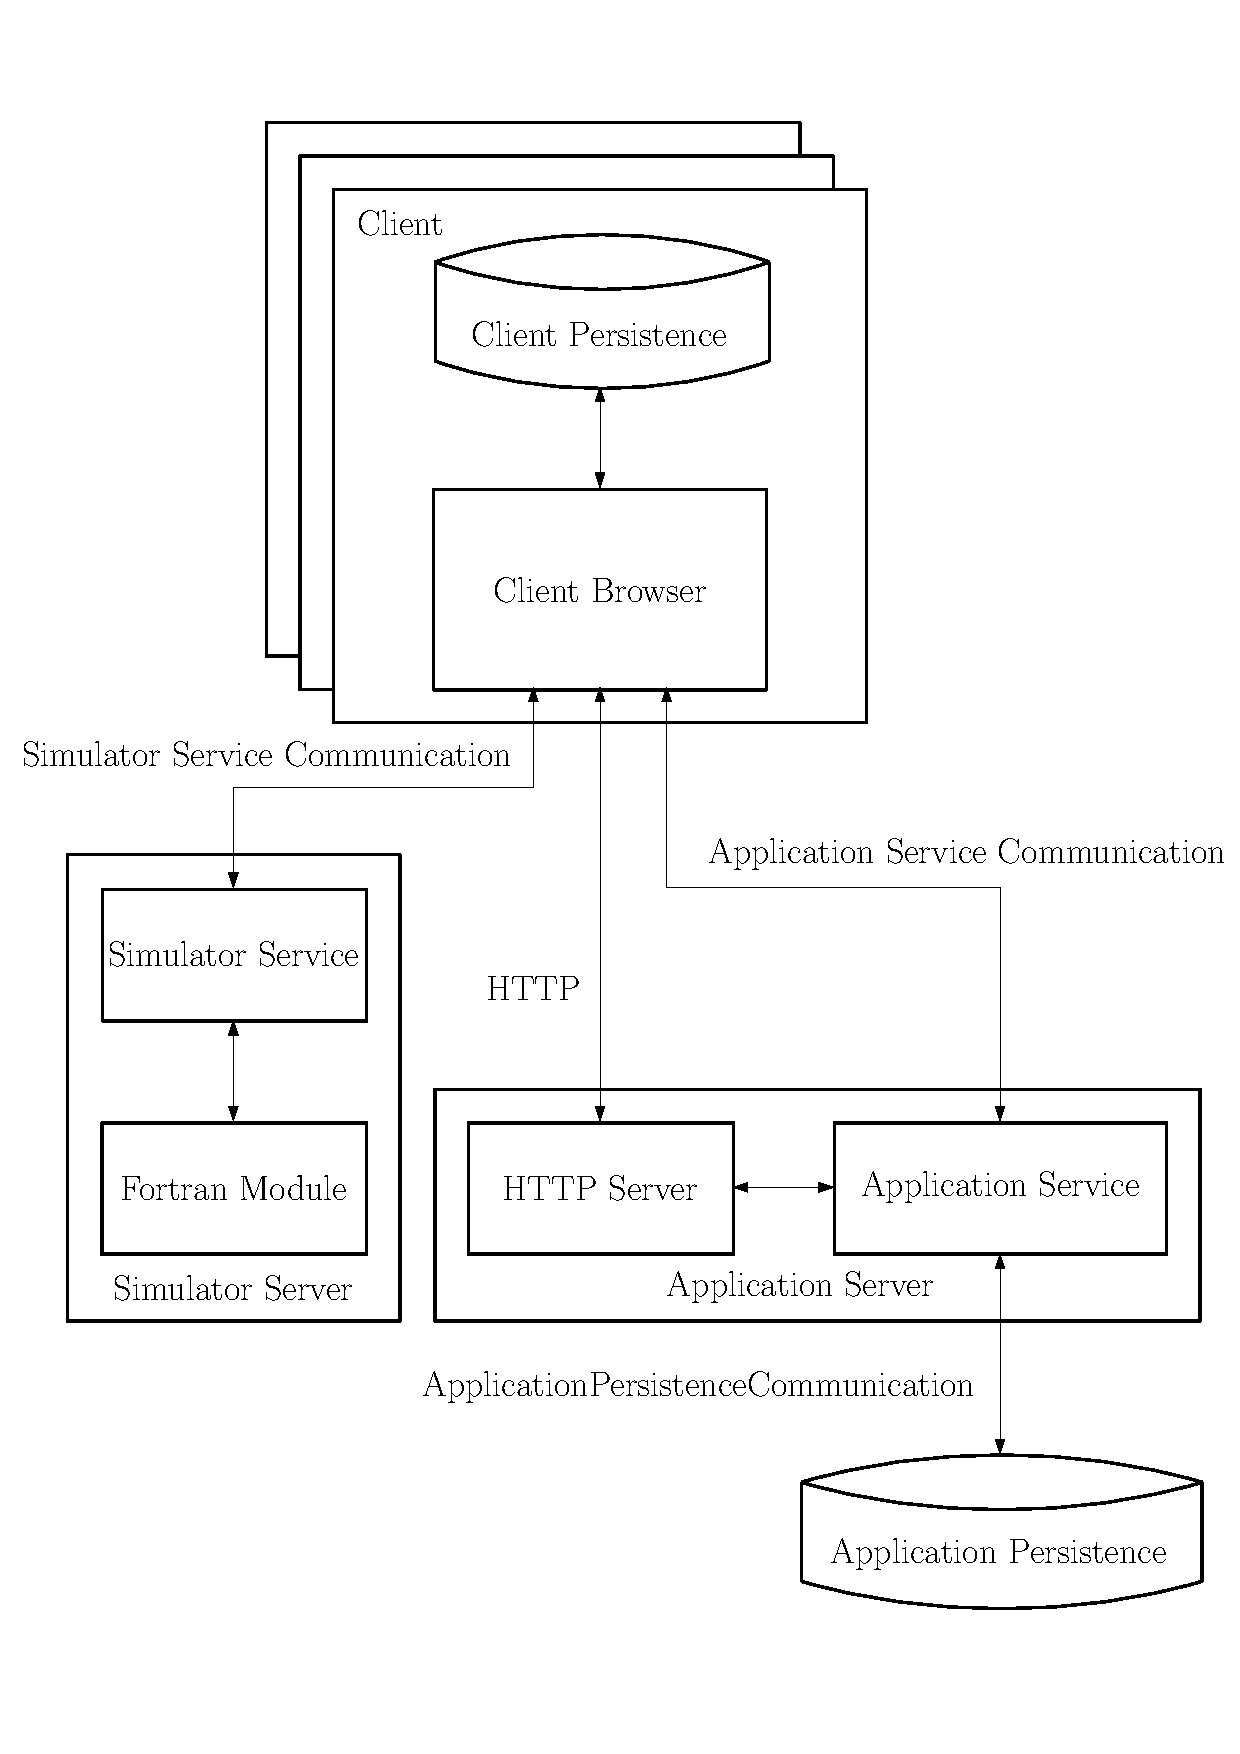
\includegraphics{SoftwareTiers}
	\caption{The different tiers of the system}
	\label{fig:tierchannel}
\end{figure}
